\chapter{Considerații teoretice și practice}
\thispagestyle{pagestyle}

\section{Medii software}
\subsection{Arduino IDE}

Arduino IDE (Integrated Development Enviroment) este un mediu de dezvoltare open source. Acesta dispune de o interfață simplă și intuitivă și de un editor de cod bazat pe limbajul de programare C/C++. Totodată, Arduino IDE beneficiază de suportul a mai multor biblioteci implementate de alți utilizatori ce acoperă o gamă largă de funcționalități, de la control de senzori și motoare până la comunicații wireless și rețialistică. Un alt avantaj al acestui IDE este compatibilitatea cu o varietate largă de plăci de dezvoltare precum Arduino Mega, Uno, Nano, NodeMCU sau orice alte plăci compatibile cu acesta \cite{arduino_ide}, \cite{arduino_ide_doc}.

\subsection{Android Studio}
Android Studio este un mediu oficial de dezvoltare pentru crearea de aplicații mobile, dezvoltat de Google și este bazat pe IntelliJ IDEA. În principal interfața oferită de acest editor este compusă din zona de editare a codului pentru limbajele de programare Java și Kotlin, manager de proiect și emulatorul Android.

Emulatorul Android permite testarea aplicațiilor pentru diferite configurații și versiuni de Android, fără a fi folosit un dispozitiv fizic. Acesta suportă diferite configurații atât hardware cât și software, astfel oferă utilizatorilor o plajă largă de teste referitoarea la comportamentul aplicațiilor în diverse condiții \cite{android_studio_doc}.


\subsection{Blynk}
Blynk este un mediu software ce facilitează dezvoltarea aplicațiilor de tip IoT (Internet of Things). Acesta permite crearea de aplicații mobile și web pentru a monitoriza și controla dispozitive hardware prin intermediul internetului. Platforma este compatibilă cu o varietate de plăci de dezvoltare precum  Arduino, Raspberry Pi, ESP8266 și NodeMCU. 

Blynk oferă biblioteci predefinite ce permit integrarea rapidă cu platfomele hardware, folosind doar un token de autentificare. Platforma pune la dispoziția utilizatorului o gamă largă de widget-uri precum butoane, gauge-uri, slider-e, display-uri și grafice, cu ajutorul cărora utilizatorul va crea o interfață potrivită nevoilor acestuia \cite{blynk_doc}. 

\subsection{EasyEDA}
EasyEDA este o platformă destinată proiectării de circuite electronice și PCB-uri (Printed Circuit Boards). Este un instrument online, dar și local, ce oferă posibilitatea de a crea și simula proiecte electronice. Platforma are integrat și un simulator SPICE unde utilizatorii pot analiza comportamentul și rezultatele circuitului.

Acesta include un editor de schemă electronică, ce permite utilizatorului să creeze diagrame și arhitecturi de circuit. EasyEDA dispune de o bibliotecă vastă de componente electronice, atât oficiale cât și create de utilizatori, incluzând modele pentru componente comune, dar și piese comerciale. De asemenea, utilizatorii, pot să creeze și să partajeze  propriile modele de componente \cite{easyEda_doc}.


\section{Protocoale Și Standarde}
\subsection{UART}
Protocolul UART (Universal Asynchronous Receiver-Transmitter) este unul dintre cele mai folosite protocoale de comunicare între două dispozitive, utilizat frecvent în electronică și informatică facilitând schimbul de date. Acest protocol permite stabilirea comunicării directe hardware printr-un canal serial. Transmisia este asincronă, ceea ce înseamnă că datele sunt transmise fără un semnal de tact comun între emițător și receptor.

\begin{figure}[H]
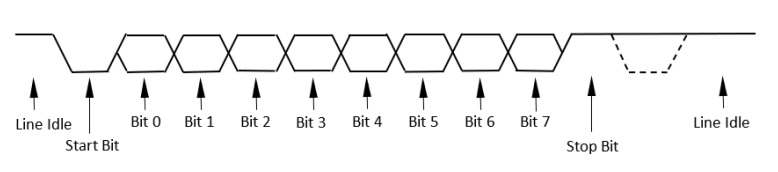
\includegraphics[width=0.8\textwidth]{images/uart_protocol.png}
\caption{Formatul de date UART \cite{uart_poza}}
\label{fig:uart_protocol}
\end{figure}

Pentru realizarea transferului de date este folosit conceptul fundamental al acestui protocol, transmisia bit cu bit secvențială. Datele au un format special, specific, ce include un bit de start ce indică începutul comunicării, în mod configurabil între 5 și 9 biți de date. Un bit de paritate ce este opțional și este folosit în verificare erorilor de transmisie și unul sau doi biți de stop care marchează sfârșitul comunicării și semnalează receptorului că biții au fost transmiși cu succes. O altă caractersitică a transferuli este viteza acestuia (baud rate-ul). Aceasta reprezintă numărul de biți transmiși pe secundă și ia valori comune precum 9600, 38400 și 115200 în funcție de nevoile și performanța sistemului. De menționat este faptul că pe ambele dispozitive se impune folosirea aceleiași viteze de transfer. \cite{pena2020uart}. 

\subsection{I2C}
Protocolul I2C (Inter-Integrated Circuit) este un protocol de comunicație serială sincronă și este utilizat pentru comunicații pe distanțe scurte. Acesta permite ca mai multe dispozitive să fie conectate simultan la o singură magistrală de comunicație și funcționează folosind o arhitectură master-slave. În mod uzual, este folosit pentru a conecta la un microcontroller,  dispozitivele  de tip slave.

\begin{figure}[H]
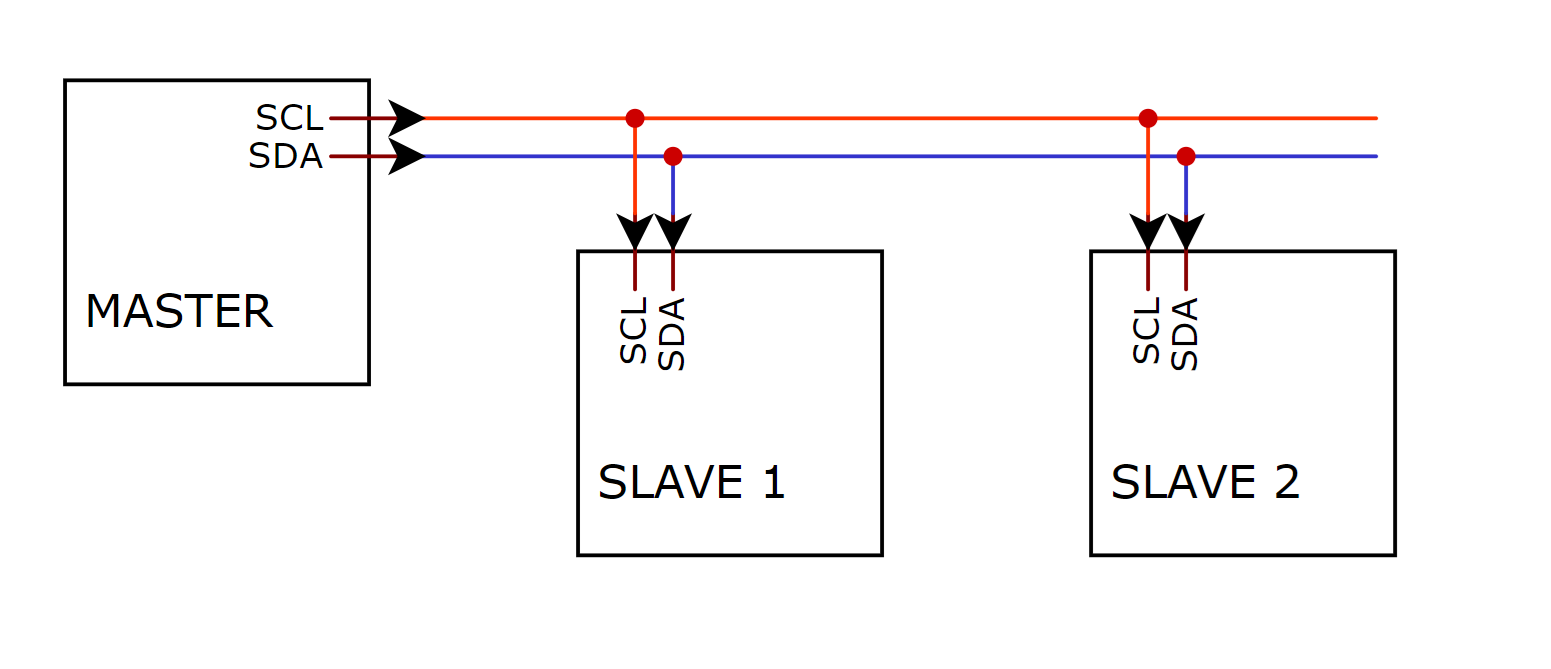
\includegraphics[width=0.7\linewidth]{bachelors_ro/images/i2c_com.png}
\caption{Conectarea dispozitivelor la magistrala I2C}
\label{fig:i2c_com}
\end{figure}

Pentru a realiza comunicarea sunt necesare două linii: SDA (Serial Data Line) și SCL (Serial Clock Line). SCL reprezintă linia de tact ce sincronizează transferul de date, iar SDA linia de date prin care se realizează transferul bidirecțional, dar nu simultan. Master-ul va furniza semnalul de tact. Dispozitivele slave au adrese unice pe magistrala I2C. Astfel, master-ul poate să comunice selectiv cu oricare dintre dispozitivele slave \cite{xu2023design}.

\subsection{Bluetooth}
Bluetooth este un standard de comunicație wireless destinat schimbului de date pe distanțe scurte până în 10 metri. Acesta folosește unde radio la o frecvență de 2.4 GHz. Dispozitivele ce beneficiază de tehnologia Bluetooth se pot conecta la alte dispozitive asemenea atât timp cât respectă raza de comunicare. În timp ce cele două dispozitive sunt conectate, acestea formează o rețea numită piconet. Interconectarea a două sau mai multe rețele piconet duce la formarea unei rețele Scatternet.

În general rata de transfer este cuprinsă între 700 kbps și 3 Mbps pentru versiunile mai vechi, iar pentru versiuni mai noi se poate ajunge până la 25 Mbps. Totodată, transmisia dispune de criptare pentru a preveni interceptarea datelor și de autentificare printr-un cod PIN sau o cheie criptografică \cite{bisdikian2001overview}.

\subsection{WiFi}
WiFi este o tehnologie ce permite conectarea dispozitivelor la internet fără a utiliza cabluri. Principiul de funcționare al WiFi-ului este bazat pe unde radio pentru a transmite date între un punct de acces (sau router) și dispozitivele conectate. Acesta folosește unde radio în banda de frecvență cuprinsă între 2.4 GHz și 5 GHz. Aceste frecvențe sunt folosite pentru a asigura o comunicare eficientă și lipsită de interferențe \cite{chernukhin2014new}.

WiFi utilizează standarde de comunicație precum IEEE 802.11, ce definește modul de transmisie și recepție al datelor. Routerele WiFi folosesc adrese IP pentru a identifica și comunica cu dispozitivele din rețea. DHCP (Dynamic Host Configuration Protocol) este utilizat adesea pentru a atribui în mod automat adrese IP dispozitivelor din rețea. Totodată, WiFi utilizează diverse metode de criptare a datelor transmise, cum ar fi WEP, WPA și WPA2 \cite{hiertz2010ieee}.

\section{Echipamente Hardware}

\subsection{Arduino Mega}
Arduino Mega 2560 R3 este echipată cu microcontrollerul ATmega2560, care oferă o capacitate mare de memorie și mai mulți pini GPIO, făcând-o ideală pentru proiecte avansate ce necesită multiple conexiuni și funcționalități complexe. Placa este compatibilă cu o varietate de shield-uri și module \cite{mega_datasheet}.

\begin{figure}[H]
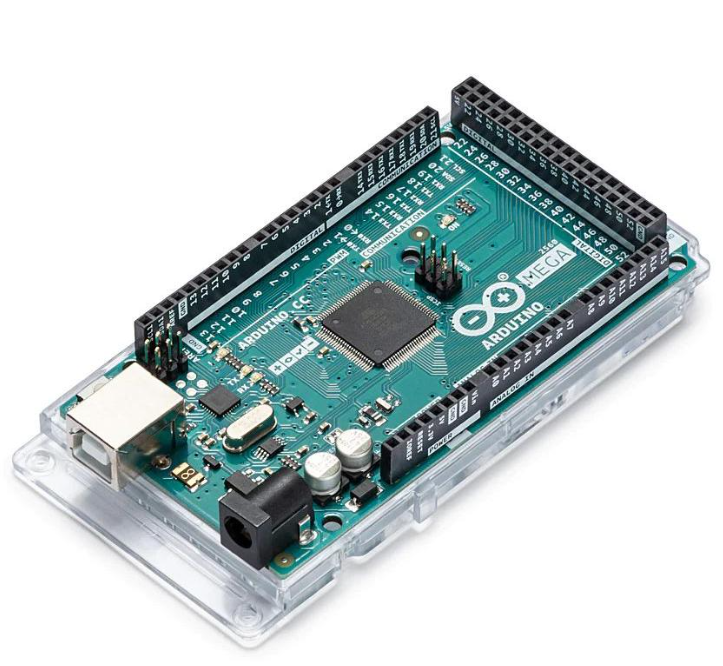
\includegraphics[width=0.7\linewidth]{images/arduino_mega.png}
\caption{Placa de dezvoltare Arduino Mega \cite{mega_poza}}
\label{fig:arduino_mega}
\end{figure}

Specificații tehnice \cite{mega_datasheet}:

\begin{itemize}
  \item Dimensiune placă 101 x 53 mm, greutate 37 g
  \item Tensiunea de alimentare este cuprinsă între 7-12 V
  \item Pini digitali 54, pini analogici 16
  \item Memorie flash de 256 KB din care 8 KB sunt utilizați de bootloader
  \item EEPROM 4 KB
  \item SRAM 8 KB
  \item Frecvența ceas 16 MHz
  \item Oferă și comunicare I2C, USB, SPI, UART
\end{itemize}

\section{Microcontroller-ul ATmega2560}
Microcontroller-ul ATmega2560 dispune de un procesor pe 8 biți din familia AVR, creat de Atmel. AVR este o arhitectură Harvard modificată. Arhitectura este pe 8 biți și este de tip RISC (Reduced Instruction Set Computer). Aceasta este cunoscută pentru eficiența sa energetică și performanța sa când vine vorba de sisteme integrate.

\begin{figure}[H]
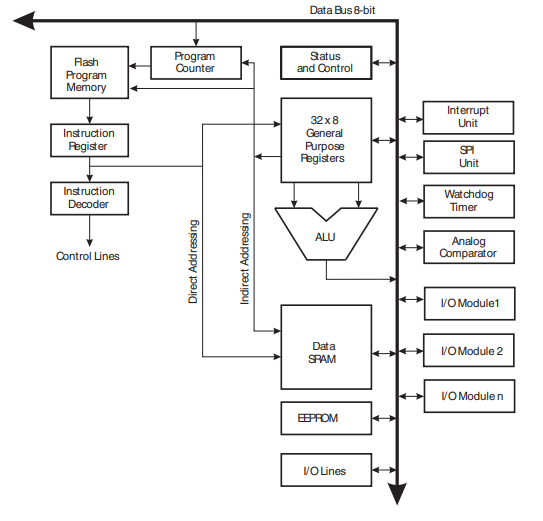
\includegraphics[width=0.6\linewidth]{bachelors_ro/images/arhitectura_avr.png}
\caption{Schema bloc a arhitecturii AVR \cite{avr_atmega2560}}
\label{fig:arhitectura_avr}
\end{figure}

Unitatea centrală de procesare (CPU) AVR este partea cea mai semnificativă a micrcontroller-ului. CPU-ul este comandat de un ceas intern ce funcționează la 16 MHz. Instrucțiunile din memoria de program sunt executate cu ajutorul unui pipeline pe un singur nivel. Astfel, în timp ce o instrucțiune este executată următoare instrucțiune este deja adusă din memoria de program. În Figura \ref{fig:instruction_pipeline} se poate observa cum are loc acest proces. Acestă metodă de bază de pipielining este folosită pentru a obține până la 1 MIPS pe MHz \cite{avr_atmega2560}.

\begin{figure}[H]
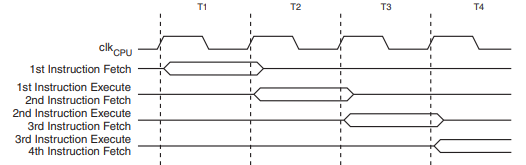
\includegraphics{bachelors_ro/images/instruction_pipeline.png}
\caption{Executarea și aducerea din memorie în paralele executată de procesor \cite{avr_atmega2560}}
\label{fig:instruction_pipeline}
\end{figure}

Această metodă permite ca în fiecare ciclu de tact să fie executată câte o instrucțiune\cite{avr_atmega2560}. Deși mai puțin eficient ca celelalte variante de pipeline, această implementare oferă siguranță împotriva apariției hazardurilor.

\subsection{Modul NodeMCU Lua WIFI ESP8266 CP2102}
NodeMCU ESP8266 este o placă de dezvoltare ce integrează modulul ESP8266, un cip WiFi cu un microcontroler integrat. Aceasta este cunoscută pentru dimensiunile compacte și capacitatea de a oferi o soluție pentru proiectele IoT (Internet of Things). NodeMCU poate fi programat utilizând chiar Arduino IDE și sunt disponibile foarte multe biblioteci pentru acesta\cite{nodemcu_datasheet}.

\begin{figure}[H]
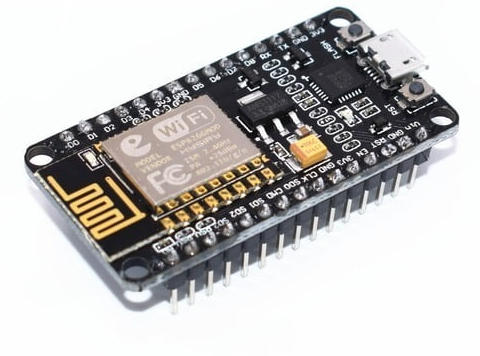
\includegraphics[width=0.5\textwidth, height=0.4\textwidth]{images/nodemcu.png}
\caption{Modul NodeMCU WIFI ESP8266 \cite{nodemcu_poza}}
\label{fig:nodemcu}
\end{figure}

\subsection{Modulul de Bluetooth HC-05}
HC-05 este un modul Bluetooth destinat comunicării seriale fără fir, care permite transferul de date între două dispozitive prin intermediul protocolului Bluetooth. Acesta poate funcționa atât în modurile master, cât și slave, ceea ce înseamnă că poate iniția conexiuni sau poate răspunde la conexiuni inițiate de alte dispozitive. Datele trimise sau primite de acest modul nu necesită nicio decodificare deoarece acestea sunt recepționate bit cu bit.

\begin{figure}[H]
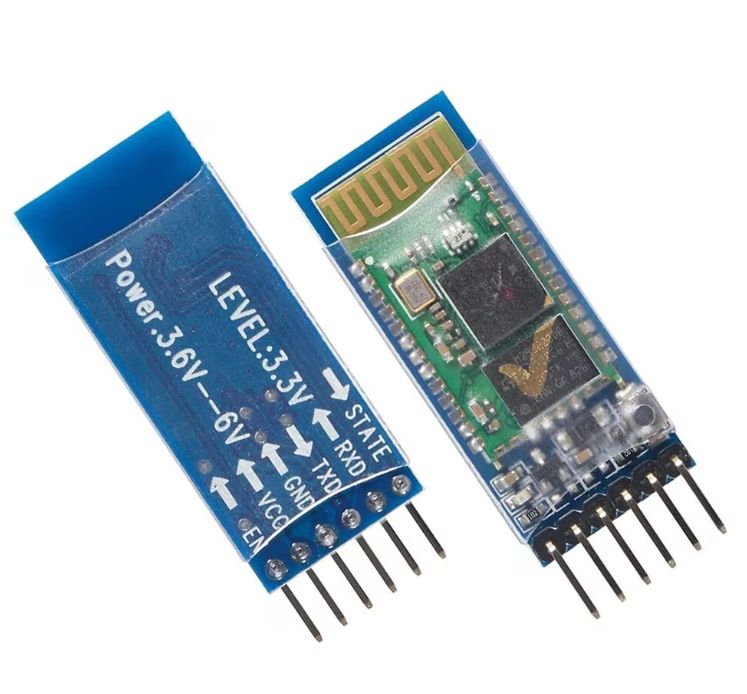
\includegraphics[width=0.3\linewidth]{images/hc05.png}
\caption{Modul Bluetooth HC-05 \cite{hc05_poza}}
\label{fig:hc05}
\end{figure}

\subsection{Display LCD 1602 cu interfață I2C}
Display-ul LCD 1602 cu interfață I2C este un afișaj cu cristale lichide, utilizat popular în proiecte de electronică. Acesta combină un ecran LCD tradițional de 16 caractere pe 2 rânduri cu un modul I2C. Reducând numărul de pini necesari pentru conexiune de la 16 la 4, simplifică integrarea în proiecte. Ținând cont că se folosește de protocolul I2C, acesta se folosește de pinii SDA și SCL pentru a recepționa date.

\begin{figure}[H]
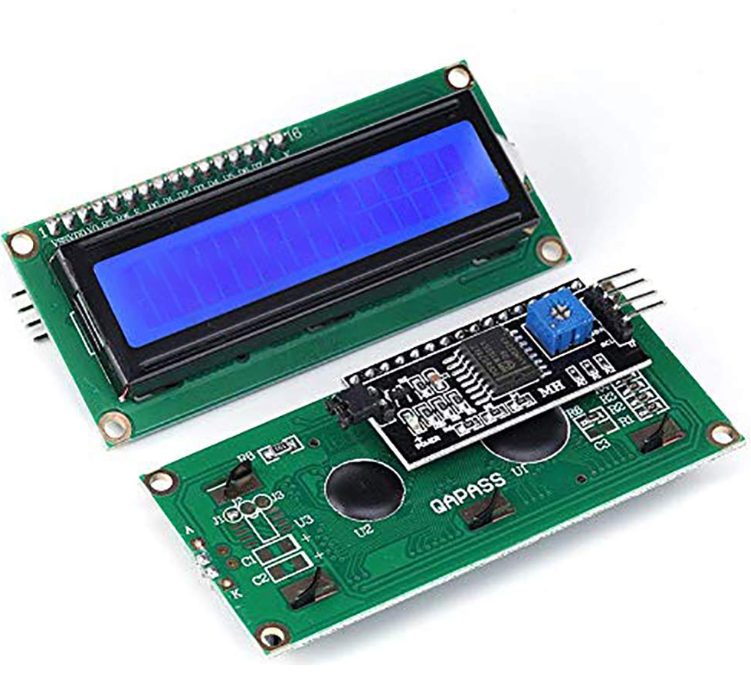
\includegraphics[width=0.4\textwidth, height=0.4\textwidth]{images/lcd.png}
\caption{Display LCD 1602 cu interfață I2C \cite{lcd_poza}}
\label{fig:lcd}
\end{figure}

\subsection{Tastatură 4x4}
Tastatură 4x4 este un keypad matricial care constă din 16 butoane dispuse în formă de matrice. Fiecare buton are o poziție unică, identificată de rândul și coloana sa. Tastatura este de obicei conectată la un microcontroler sau la un alt dispozitiv de control, care citește stările butoanelor pentru a detecta apăsările de taste.

\begin{figure}[H]
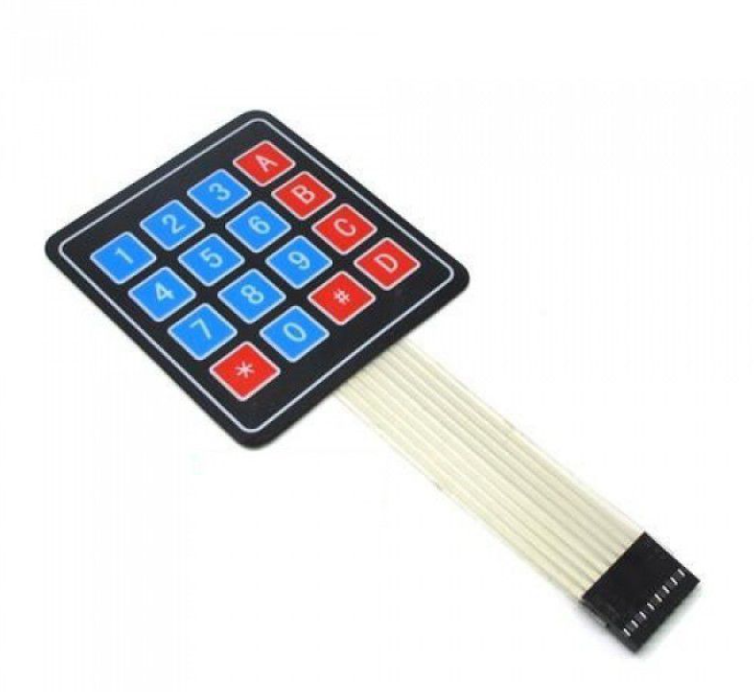
\includegraphics[width=0.4\textwidth, height=0.4\textwidth]{images/tastatura.png}
\caption{Tastatură 4x4 \cite{key_poza}}
\label{fig:tastatura}
\end{figure}


\subsection{Modul Releu}
Un releu este un dispozitiv electric ce funcționează ca un întrerupător, fiind controlat de un circuit electronic. Acesta este utilizat pentru a gestiona circuite de înaltă putere prin intermediul unui semnal de joasă putere. Releul este alcătuit din două componente esențiale: un electromagnet și un set de contacte. Atunci când o tensiune de control este aplicată electromagnetului, se generează un câmp magnetic care acționează asupra unui comutator mecanic, permițând deschiderea sau închiderea circuitului electric.

\begin{figure}[H]
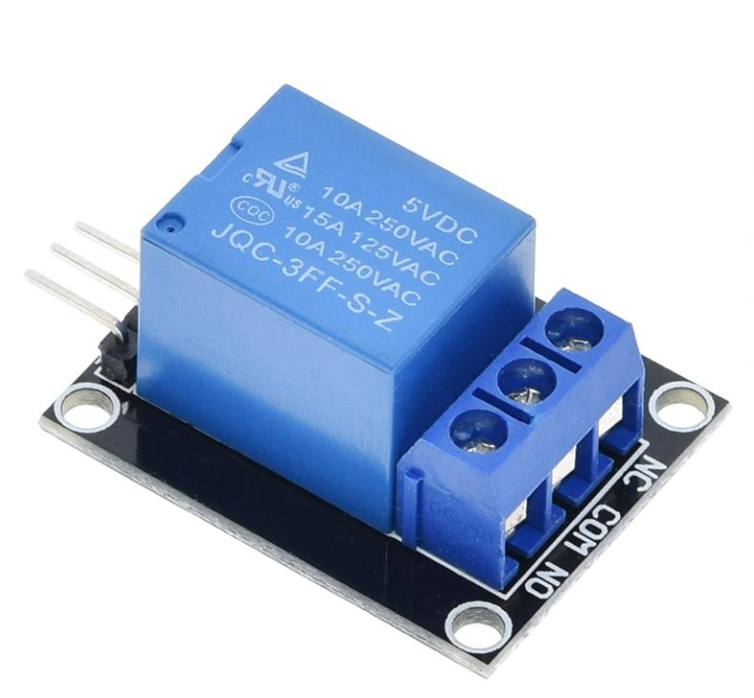
\includegraphics[width=0.3\textwidth, height=0.3\textwidth]{images/releu.png}
\caption{Modul releu cu un singur canal\cite{releu_poza}}
\label{fig:releu}
\end{figure}

\subsection{Senzori}
BMP280 este un senzor de înaltă precizie pentru măsurarea presiunii barometrice și a altitudinii. Fabricat de Bosch Sensortec, acest senzor compact și performant oferă măsurători exacte, fiind perfect pentru aplicații portabile și autonome. Utilizând tehnologia MEMS (Micro-Electro-Mechanical Systems), BMP280 se remarcă prin consumul său redus de energie și fiabilitatea sa în diverse condiții de operare.

\begin{figure}[H]
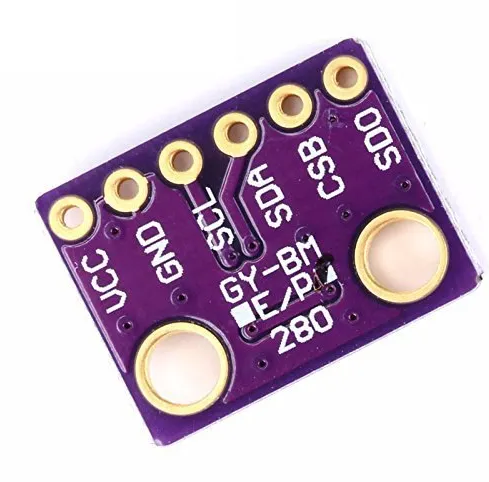
\includegraphics[width=0.3\textwidth, height=0.3\textwidth]{images/bmp.png}
\caption{Senzorul BMP280\cite{bmp_poza}}
\label{fig:bmp}
\end{figure}

DHT11 este un senzor digital folosit pentru a măsura atât temperatura, cât și umiditatea. Datorită ușurinței sale de utilizare este potrivit pentru proiecte de monitorizare a condițiilor de mediu și automatizări casei. Acest senzor integrează un termistor și un senzor capacitiv pentru umiditate, furnizând date precise în format digital.

\begin{figure}[H]
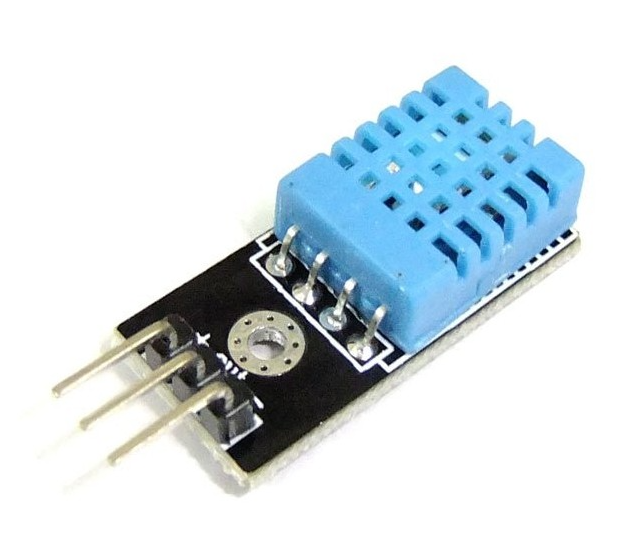
\includegraphics[width=0.3\textwidth, height=0.3\textwidth]{images/dht11.png}
\caption{Senzorul DHT11\cite{dht_poza}}
\label{fig:dht11}
\end{figure}

Senzorul MQ-2 este conceput pentru a detecta concentrații de gaze inflamabile, inclusiv propan, butan, metan și hidrogen, precum și fum. Acest senzor folosește un element sensibil din oxid de staniu (SnO2), care își reduce rezistența electrică în prezența acestor gaze, permițând astfel măsurarea concentrației de gaz.

\begin{figure}[H]
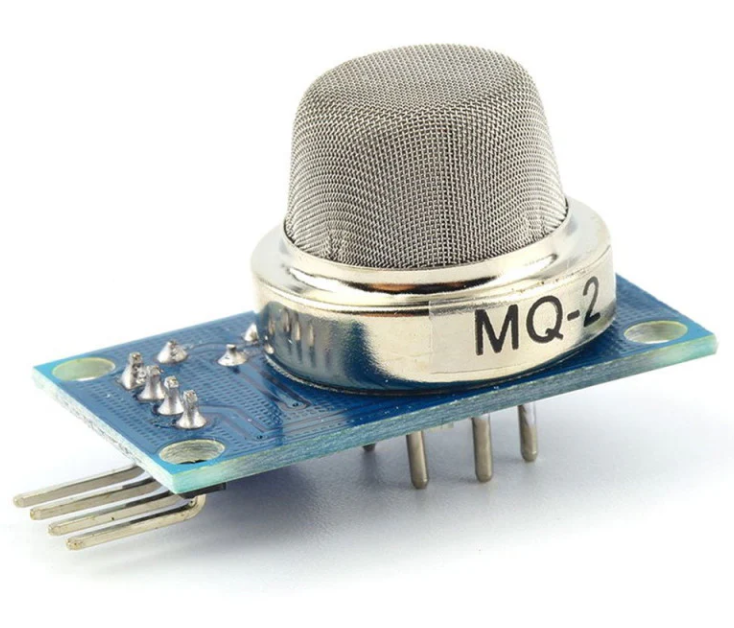
\includegraphics[width=0.3\textwidth, height=0.3\textwidth]{images/mq2.png}
\caption{Senzorul MQ2\cite{mq_poza}}
\label{fig:mq2}
\end{figure}

Un modul cu fotorezistor constă într-un fotorezistor și un circuit de bază, ce include un potențiometru pentru reglarea sensibilității, precum și conexiuni pentru alimentare și transmiterea unui semnal digital . Fotorezistorul, componenta esențială a modulului, își modifică rezistența în funcție de nivelul de lumină la care este expus, permițând astfel generarea unui semnal digital corespunzător.

\begin{figure}[H]
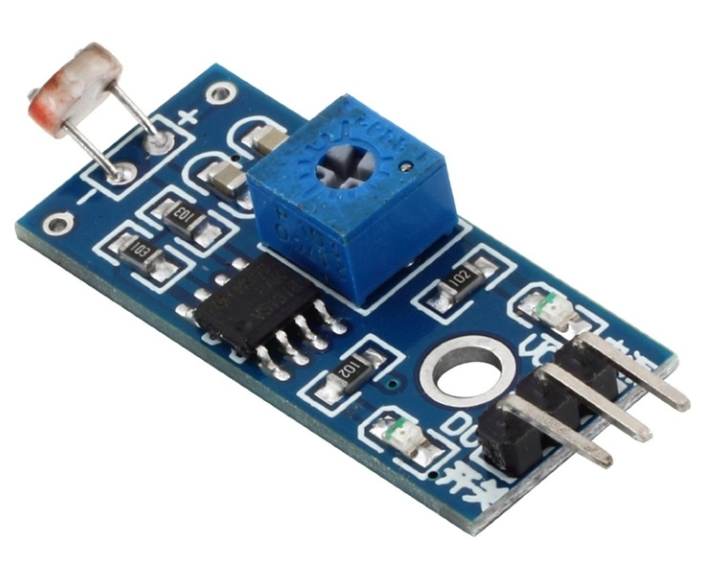
\includegraphics[width=0.3\textwidth, height=0.3\textwidth]{images/senz_lumina.png}
\caption{Modul cu fotorezistor\cite{senzlum_poza}}
\label{fig:senz_lumina}
\end{figure}

HC-SR501 este un senzor PIR (Passive Infrared) care identifică mișcarea detectând modificările în radiația infraroșie din mediul înconjurător. Acesta include un element detector de infraroșu, un circuit de procesare și o lentilă Fresnel, care focalizează radiația infraroșie pe elementul sensibil. Atunci când un obiect cu o temperatură diferită față de fundal (cum ar fi o persoană sau un animal) se deplasează în zona de detectare, senzorul emite un semnal de ieșire.

\begin{figure}[H]
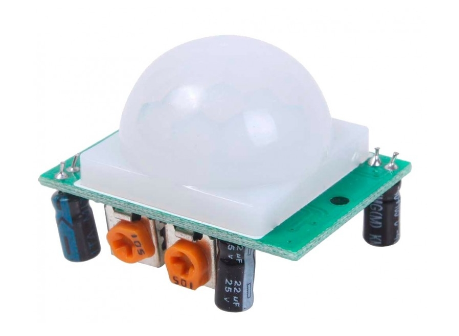
\includegraphics[width=0.4\linewidth]{images/pir.png}
\caption{Senzorul HC-SR501 PIR\cite{pir_poza}}
\label{fig:pir}
\end{figure}

HC-SR04 este un senzor ultrasonic destinat măsurării distanței. Acest senzor funcționează prin emiterea undelor ultrasonice pentru a determina distanța față de un obiect. Are patru pini: VCC, Trig, Echo și GND. Senzorul generează un impuls ultrasonic de 40 kHz prin intermediul pinului Trig și primește ecoul reflectat prin pinul Echo. Intervalul de timp necesar pentru ca semnalul să se reflecte înapoi este utilizat pentru a calcula distanța față de obiectul detectat.

\begin{figure}[H]
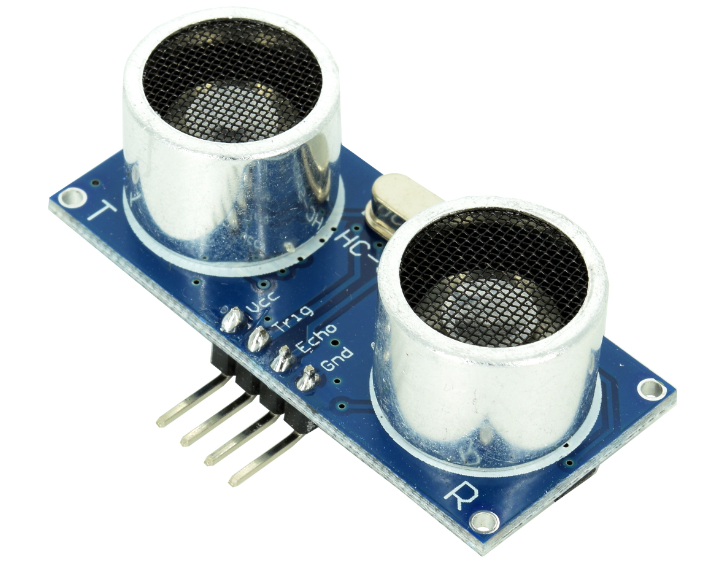
\includegraphics[width=0.4\textwidth, height=0.3\textwidth]{images/ultrasonic.png}
\caption{Senzorul HC-SR04\cite{ultras_poza}}
\label{fig:ultrasonic}
\end{figure}


\subsection{Microservo SG90}
Microservo SG90 este un servomotor compact, care operează utilizând semnale PWM (Pulse Width Modulation). Arborele său de ieșire poate fi reglat la unghiuri cuprinse între 0 și 90 de grade. Acest reglaj se realizează prin modificarea semnalului PWM trimis motorului. Microservo SG90 include un motor DC de mici dimensiuni, un set de angrenaje pentru reducerea vitezei și creșterea cuplului, precum și un circuit de control. Circuitul de control interpretează semnalul PWM de la microcontroller și ajustează poziția arborelui în funcție de durata impulsurilor semnalului.

\begin{figure}[H]
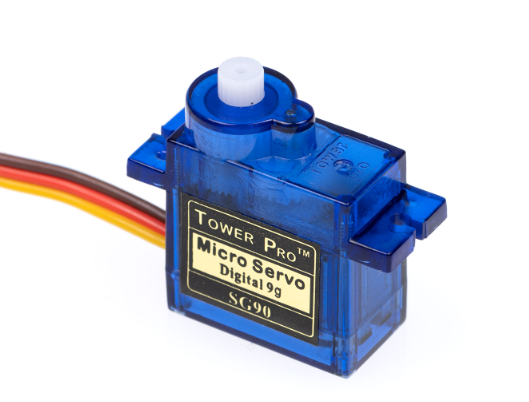
\includegraphics[width=0.4\textwidth, height=0.3\textwidth]{images/servo.png}
\caption{Microservo SG90\cite{servo_poza}}
\label{fig:servo}
\end{figure}

\subsection{Buzzer pasiv și LED}
Buzzerele pasive sunt dispozitive care produc sunet atunci când primesc un semnal cu frecvență variabilă. Acestea transformă semnalul electric în vibrații mecanice, generând astfel unde sonore. Spre deosebire de buzzerele active, cele pasive sunt mai versatile, fiind capabile să emită o varietate de tonuri și sunete în funcție de semnalul de control primit.

\begin{figure}[H]
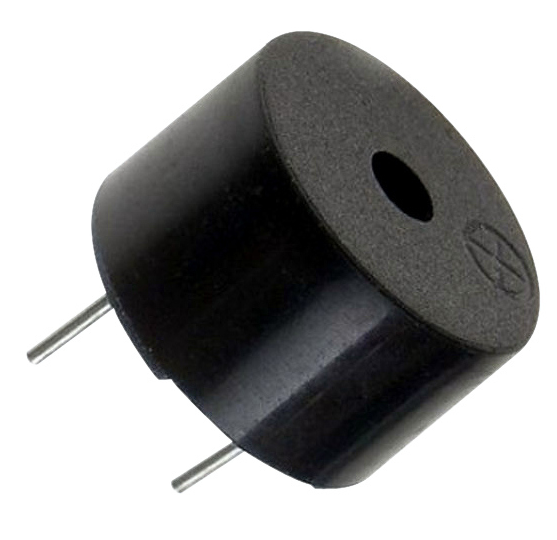
\includegraphics[width=0.3\textwidth, height=0.3\textwidth]{images/buzzer.png}
\caption{Buzzer Pasiv\cite{buzzer_poza}}
\label{fig:buzzer}
\end{figure}

LED-urile sunt diode care emit lumină atunci când un curent electric le parcurge într-o anumită direcție. Acestea sunt disponibile într-o varietate de culori, dimensiuni și forme, fiind utilizate în numeroase aplicații, de la iluminat interior și exterior, până la afișaje digitale, semnalizări și dispozitive electronice. Comparativ cu becurile tradiționale, LED-urile nu au filament și generează foarte puțină căldură, ceea ce le conferă o eficiență energetică superioară.

\begin{figure}[H]
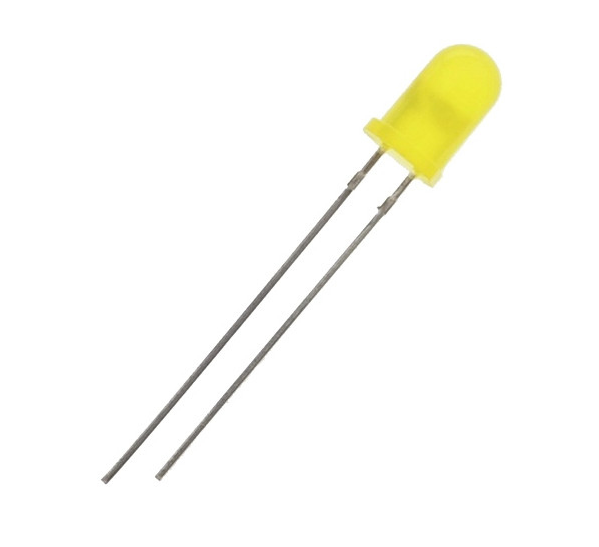
\includegraphics[width=0.3\textwidth, height=0.3\textwidth]{images/led.png}
\caption{LED\cite{led_poza}}
\label{fig:led}
\end{figure}

\subsection{Sursă alimentare 12 V, Ventilator și bec H7}
O sursă de alimentare care convertește tensiunea de 220V AC la 12V DC funcționează prin mai multe etape cheie. În prima fază, curentul alternativ de 220V este transformat în curent continuu pulsatoriu prin intermediul unui circuit redresor, de obicei un pod redresor. Apoi, acest curent continuu pulsatoriu este netezit de un condensator de filtrare, producând un curent continuu mai stabil. Următoarea etapă implică reducerea și stabilizarea tensiunii la 12V folosind un regulator de tensiune sau un convertor DC-DC step-down. De asemenea, sursa de alimentare include circuite de protecție care previn deteriorările cauzate de supratensiuni, scurtcircuite sau supraîncălziri. Toate aceste procese sunt integrate într-un circuit compact, oferind o conversie eficientă și stabilă a tensiunii pentru a asigura funcționarea în siguranță și fiabilitatea dispozitivelor conectate.

\begin{figure}[H]
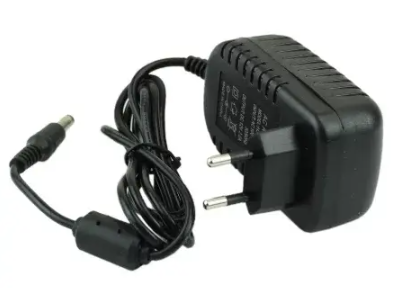
\includegraphics[width=0.4\textwidth, height=0.3\textwidth]{images/sursa.png}
\caption{Sursă de alimentare\cite{sursa_poza}}
\label{fig:sursa}
\end{figure}

Un ventilator funcționează prin convertirea energiei electrice în energie mecanică pentru a produce un flux de aer. Alimentat la o tensiune de 12V DC, motorul electric, adesea de tip brushless, transformă energia electrică în mișcare, rotind axul pe care sunt fixate palele ventilatorului. Această rotație generează un curent de aer, a cărui direcție și intensitate depind de designul și viteza palelelor. Viteza ventilatorului poate fi ajustată manual printr-un controler sau automat, cu ajutorul unui senzor de temperatură.

\begin{figure}[H]
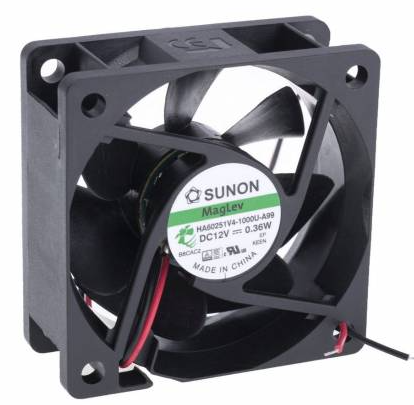
\includegraphics[width=0.3\textwidth, height=0.3\textwidth]{images/ventilator.png}
\caption{Ventilator 12 V\cite{vent_poza}}
\label{fig:ventilator}
\end{figure}

Becul H7 este larg utilizat în sistemele de iluminat auto, fiind recunosccut pentru farurile de fază scurtă și lungă. Acest tip de bec aparține categoriei de becuri halogen și este recunoscut pentru luminozitatea și claritatea luminii pe care o oferă.

Aceste becuri funcționează pe baza principiului halogenului, unde un filament de tungsten este înconjurat de un gaz halogen. Acest design permite becurilor să aibă o durată de viață mai lungă și o temperatură de operare mai mare în comparație cu becurile incandescente tradiționale. Rezultatul este o lumină mai strălucitoare și mai albă, care îmbunătățește vizibilitatea pe timp de noapte și în condiții meteorologice dificile.

\begin{figure}[H]
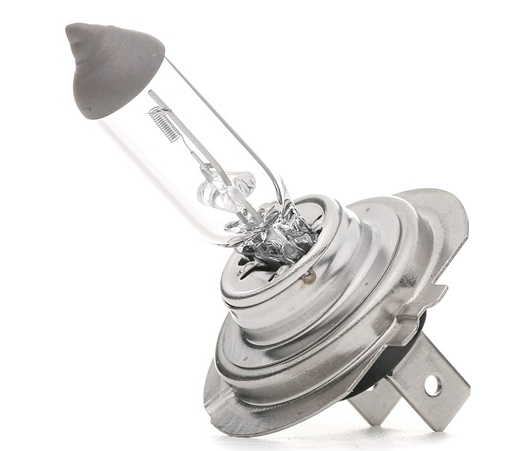
\includegraphics[width=0.3\textwidth, height=0.3\textwidth]{images/bec_h7.png}
\caption{Bec H7\cite{bech7_poza}}
\label{fig:bec_h7}
\end{figure}


